\problem{What are the required properties to check whether the given function is lossless oneport network function or not? Explain with examples.}
The properties that are required to check if a given function is lossless oneport network function are,
\begin{enumerate}
    \item The driving point function, (impedance function or admittance function), $Z(s)$ or $Y(s)$ is the ratio of even polynomial to odd polynomial degree or vice versa.
    \item There must be either a pole or zero at origin and infinity.
    \item The highest degree of numerator and denominator must differ by at most unity. Similar condition is necessary for the lowest power.
    \item The succeeding powers of both numerator and denominator polynomials must differ by two. 
    \item All the poles and zeros must lie on the imaginary axis and must alternate.
    \item The reciprocal of a lossless circuit is also lossless.
\end{enumerate}
An important point to note is that if the poles and zeros lie on the imaginary axis and they alternate, then it is the sufficient condition for the function to be lossless oneport network.
Let us assume two driving point functions as,
\begin{equation*}
    Z_1(s)=\frac{5(s^2+1)(s^2+9)}{(s^2+4)(s^2+12)} \quad   Z_2(s)=\frac{2(s^2+1)(s^2+9)}{s(s^2+4)}
\end{equation*}
Here, $Z_1(s)$ is not the ratio of even polynomial to odd polynomial, so it is simply rejected and hence is not a valid lossless function. However, $Z_2(s)$ is a ratio of even polynomial to odd polynomial, so it may be valid lossless function. We need to check the poles and zero plot as,
\begin{figure}[H]
    \centering
    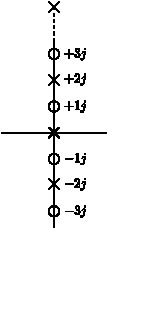
\includegraphics[scale=1.5]{../Figures/pole_lc}
    \caption{Pole and zero location for $Z_2(s)$}
    \label{fig:pole-lc-2}
\end{figure}